\chapter{Theoretical Background and Methodology}
\justifying
Understanding the evolution of a multi-component system consisting of hundreds or thousands of atoms is typically performed using Molecular Dynamics (MD) simulations, where we simulate the motion of the particles at discrete time steps by solving Newton's equations of motion. MD simulations involve the generation of a 3N-dimensional potential energy surface at every time slice, and the energy derivatives at each step are employed to propagate the coordinates and velocities to the next step. The same, using mathematical expressions, can be expressed as follows:
\begin{multline*}
    V(r^N) = \sum_{bonds}^{}k_i(x_i-x_i^{min})^2 + \sum_{angles}^{}k_j(\theta_i-\theta_i^{min})^2 + \sum_{dihedrals}^{}k_{\phi}(1 + cos(n\phi-\delta)) + \\ \sum_{impropers}^{} k_{\omega}(\omega - \omega_{min})^2 + \sum_{UreyBradley}^{}(S-S_{min})^2 + \\ \sum_{electrostatic}^{}\frac{1}{\epsilon}*\frac{q_i * q_j}{r_{ij}} +  \sum_{VdW}^{}\epsilon_{ij}(\frac{\sigma_{ij}^{12}}{r_{ij}^2}-\frac{\sigma_{ij}^{6}}{r_{ij}^6})
\end{multline*}
\begin{equation*}
    F_i =   -\frac{\delta V}{\delta r_i}
\end{equation*}

The equation $F = m*a$ as a matrix equation where $F$ is a matrix of dimensions (natoms, 3) and mass is avector of dimensions (natoms, 1). Thus, accelarations for all particles at each step is evaluated as $a = F \backslash m$, solving a system of linear equations at each step. Once the accelarations for time step $t$ are generated, the positions and velocities are propagated to the next using one of the many algorithms described below:
\begin{enumerate}
    \item \textbf{Verlet algorithm}: The Verlet algorithm is a second-order integrator where the positions and velocities are propagated through time, starting from an initial set of coordinates and velocities. The Verlet algorithm is a numerically stable method. The algorithm is time reversible, meaning it is possible to run the integrator backwards to identify the dynamical trajectory's starting position due to the equations' lack of randomness. The basic algorithm does not require knowledge about the particle velocities to propagate the coordinates through time due to the algorithm's structure, which has a form described below.
    \begin{align*}
        x(1) &= x(0) + v(0)*\Delta t + \frac{1}{2}a(0)\Delta{t^2} \\
        x(t+1) &= 2x(t) - x(t-1) + a(t)\Delta{t^2}
    \end{align*}
    \item \textbf{Velocity-Verlet algorithm}: Velocity-verlet algorithm has explicit dependence on the velocities of the particles, and we use the velocities calculated at the midpoint of two consecutive timesteps in propagating the coordinates through time. The equations governing the Velocity-verlet algorithm have the form described below.
    \begin{align*}
        v(t + \frac{1}{2}\Delta{t}) &= v(t) + \frac{1}{2}a(t)\Delta{t} \\
        x(t+1) &= x(t) + v(t+ \frac{1}{2}\Delta{t})\Delta{t} \\
        a(t+1) &= F(t)/m \\
        v(t+1) &= v(t+\frac{1}{2}\Delta{t}) + \frac{1}{2}a(t+\Delta{t})\Delta{t}
    \end{align*}
    \item \textbf{Leapfrog algorithm}: The Leapfrog algorithm is conceptually similar to the Velocity-verlet method in that positions and velocities leapfrog over each other in sequence. Similar to Verlet and Velocity-verlet algorithms, the leapfrog algorithm is also a second-order algorithm. 
    \item \textbf{Langevin Integrator}: Langevin dynamics controls the system's temperature by introducing a Gaussian random error term, which readjusts the particles' velocities via collisions with virtual particles modelled via Gaussian random errors. However, the presence of this error term means that Langevin dynamics is not time-reversible, unlike other algorithms.
\end{enumerate}

The quality of a molecular dynamics simulation is highly dependent on multiple factors, in which three factors listed below are of significant importance:
\begin{enumerate}
    \item Initial positions of the atoms in the starting structure. If the intial confirmations introduce some baises in the system, it would affect the simulations outcomes, such that all possible states might not get adequately sampled during the simulation.
    \item Parameters used to describe the interactions between the particles (atoms) during the MD simulation, which are used to compute the potential energy surface. If the parameters used are unable to describe certain interactions, the predictions might not be reflective of the experimental observations.
    \item Integrator used to propagate the structure from time step of $t$ to time step of $t+1$. Some integrators might be numerically unstable over large lengths of time, and the errors at each step might get accumulated in the trajectory.
\end{enumerate}

Having introduced the reader to the basic theory behind MD simulations, further details regarding the Force fields (FFs) and other integration parameters are presented in the subsequent sections.
\section{Force fields}
The fundamental idea behind FFs is to decompose the interactions between collections of atoms into a set of analytic functions fitted to reproduce QM results and (or) experimental observables. We can decompose the interactions between sets of atoms into the following sections:
\begin{enumerate}
    \item We model all atoms as hard spheres, and Hook's law models the bonds between atoms, where the bond is approximated with a spring of a specified spring constant, empirically determined. 
    \item We use Hook's law to model angles between three bonded atoms, where the spring constant determines the flexibility of the angle and is also empirically determined. 
    \item We use a periodic potential to model the dihedral between four bonded atoms since the dihedral angle is between [0,180]. 
    \item The standard Lennard-Jones equation evaluates non-bonded interactions between all pairs of non-bonded atoms.
\end{enumerate}
One central assumption is that the parameters are molecule-agnostic, i.e. the parameters developed for one set of atoms can be transferred with minimal reparameterization towards another molecule, provided the chemical environment of the atom is equivalent. In other words, the parameters used to describe a carbon atom in benzene must be transferrable to describe the carbon atom in naphthalene.

We have employed Chemistry at HAR Molecular Mechanics (CHARMM) FF for the simulations reported in this thesis. The functional form of the classical non-polarizable additive FF is as follows:
\begin{multline*}
    V(r^N) = \sum_{bonds}^{}k_i(x_i-x_i^{min})^2 + \sum_{angles}^{}k_j(\theta_i-\theta_i^{min})^2 + \sum_{dihedrals}^{}k_{\phi}(1 + cos(n\phi-\delta)) + \\ \sum_{impropers}^{} k_{\omega}(\omega - \omega_{min})^2 + \sum_{UreyBradley}^{}(S-S_{min})^2 + \\ \sum_{electrostatic}^{}\frac{1}{\epsilon}*\frac{q_i * q_j}{r_{ij}} +  \sum_{VdW}^{}\epsilon_{ij}(\frac{\sigma_{ij}^{12}}{r_{ij}^2}-\frac{\sigma_{ij}^{6}}{r_{ij}^6})
\end{multline*}

where $k_i$, $k_j$ etc are the spring constants for the bonds and angles respectively. Values indicated as $x_{i}^{min}$, $\theta_{i}^{min}$ correspond to the equilibrium bond length and angle. As observed from the equation, the dihedral energy is expressed as the linear combination of a periodic cosine function, where $k_{\phi}$ is the force constant, $\phi$ is the dihedral angle, $\delta$ is the phase shift, and $n$ is the multiplicity of the dihedral. Improper dihedrals are important in maintaining the planarity of a structure, where $k_{\omega}$ is the spring constant and $\omega$ characterizes the out-of-plane bend of the plane. Urey-Bradley interactions account for the 1-3 interactions between the $i^{th}$ and $k^{th}$ atoms in an angle formed by i, j and k atoms, and has important applications in maintaining the geometry of H-O-H angle in water. VdW interactions between two non-bonded atoms i and j, separated by a distance $R_{ij}$ is evaluated using a pairwise Lennard-Jones potential dependent on the specific ``well-depth'' $(\epsilon)$ and equilibrium distance $\sigma$ for the interating particles. The energy terms are evaluated using the standard Lorentz-Berthelot mixing rules:
\begin{align*}
    \sigma_{ij} &=   \frac{\sigma_i + \sigma_j}{2} \\
    \epsilon_{ij} &= \sqrt{\epsilon_i*\epsilon_j}
\end{align*}
Electrostatic energy is computed using Coulumb potential, with $q_i$ and $q_j$ being the partial charges on the particles, and $r_{ij}$ being the distance between the particles.

We have also used classical Drude polarizable FF to investigate the influence of polarizability on the dynamics of the systems. Here, we note that classical non-polarizable FFs like CHARMM have their basis in fixed-point charges, which means that they are not particularly suited for studying systems where significant shifts in the local environment for the molecules are expected, like in the case of biological systems. In such cases, polarizable FFs like classical Drude polarizable FF offers a pathway towards the inclusion of the contributions from the local environment towards the dynamics of the systems.

In the case of classical Drude polarizable FF, the polarizability of the heavy atoms (excluding hydrogen) is modelled via Drude particles attached to the heavy atoms via a harmonic spring. The Drude particles have a negative charge associated with them. In contrast, the atomic cores have a positive charge, such that the total charge of the atom and associated Drude particle equals the partial charge of the atom. A representative structure depicting the arrangement of atomic cores and associated drude particles are presented in Figure 2.1. 
\begin{figure}
    \centering
    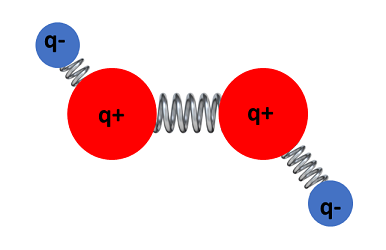
\includegraphics{Methods/Figures/drude.png}
\end{figure}

\section{Periodic Boundary Conditions}
It is computationally impractical to perform MD simulations on systems of experimentally relevant dimensions. Periodic boundary conditions (PBC) allow us to use a simulation box of computationally trackable dimensions and mitigate finite box effects like self-interactions. Under periodic boundary conditions, any particle leaving the box during the simulation is replaced by its image from one of the twenty-six periodic images generated around the original simulation box. 
\begin{figure}
    \centering
    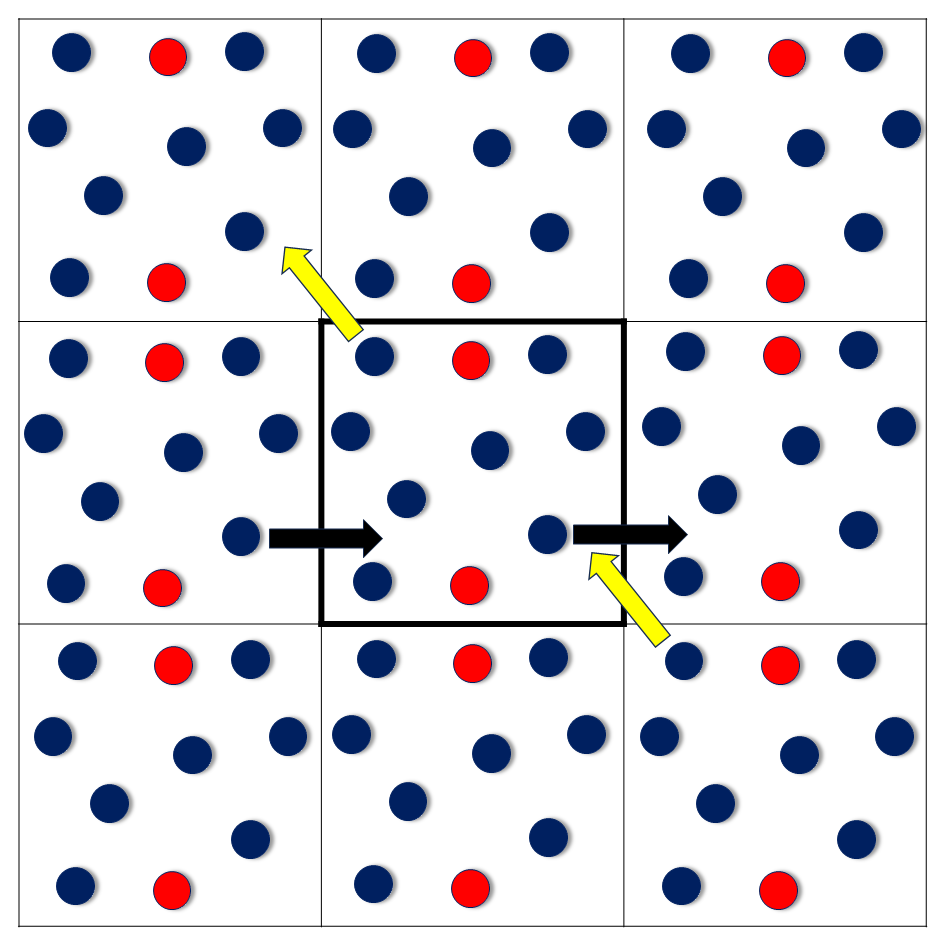
\includegraphics[width=0.75\textwidth]{Methods/Figures/pbc.png}
    \caption[Representative image depicting the application of PBC in a 2D plane]{Representative image depicting the application of PBC in a 2D plane. The central simulation box is indicated by the use of solid lines. The trajectory for two particles at the edges of the simulation box, and its periodic images are also indicated.}
\end{figure}

Consider the case of a 3D system with system dimensions of Lx, Ly and Lz and angles of 90. A naive implementation for the periodic boundary conditions, in this case, would be as follows:
\begin{align*}
    r &= r - r_{old}        \\           
    r &= r - \text{ANINT}( \frac{r}{box}) * box \\
    % r &= r + r_{old}               \\    
\end{align*}
Here $r$ and $r_{old}$ are the coordinates of the particle at time $t+1$ and $t$, and ANINT is a Fortran routine that rounds a floating point number to the nearest integer.
\section{Software and Hardware Used}
This thesis employed the Nanoscale Molecular Dynamics (NAMD) simulation package to perform all classical MD simulations. The initial QM calculations reported in the first chapter used Gaussian 09 and Orca. Home-developed Python codes were also utilized to conduct all the analyses reported herein. All MD trajectories and PDB structures were visualized using the Visual Molecular Dynamics (VMD) and GaussView packages. This thesis required extensive computational resources provided by the High-Performance Computing Facility, IIT Gandhinagar, and Param Ananta Supercomputing Facility at IIT Gandhinagar. 